\begin{center}
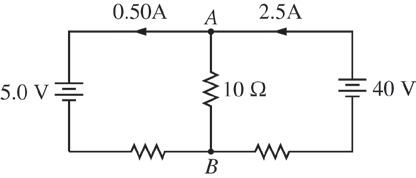
\includegraphics[scale=0.5]{images/img-002-002.png}
\end{center}

% Multiple Choice Question 2
\begin{questions}\setcounter{question}{1}\question
In the circuit shown above, a student has measured the currents that are given in the diagram, but does not know all the resistance values. The magnitude of the potential difference between points $A$ and $B$ is

\begin{oneparchoices}
\choice $10 \unit{V}$
\choice $20 \unit{V}$
\choice $30 \unit{V}$
\choice $35 \unit{V}$
\choice $40 \unit{V}$
\end{oneparchoices}\end{questions}

